\documentclass[11pt,a4paper]{article}
\usepackage[utf8]{inputenc}
\usepackage[T1]{fontenc}
\usepackage[russian]{babel}
\usepackage[a4paper,
                         left=3cm,
                         top=2cm,
                         right=1.5cm,
                         bottom=2cm,
                         marginparsep=7pt,
                         marginparwidth=.6in]{geometry}
\usepackage{amsmath}
\usepackage{amsfonts}
\usepackage{amssymb}
\usepackage{graphicx}
\usepackage{indentfirst}
\usepackage{pscyr}
\usepackage{hyperref} 
\usepackage{float}
\usepackage{minted}
\begin{document}
	\thispagestyle{empty}
	\begin{center}
		\textbf{Национальный Исследовательский Университет ИТМО}\\
		\textbf{Факультет Программной Инженерии и Компьютерной Техники}\\
	\end{center}
	\vspace{2em}
	\begin{center}
		
\includegraphics[width=120px]{../../../itmo-logo.png}
	\end{center}
	\LARGE
	\vspace{5em}
	\begin{center}
		\textbf{Вариант № 86006.15}\\
		\textbf{Лабораторная работа № 4}\\
		\Large
		\textbf{по дисциплине}\\
		\LARGE
		\textbf{\emph{'Программирование'}}\\
	\end{center}
	\vspace{11em}
	\large
	\begin{flushright}
		\textbf{Выполнил:}\\
		\textbf{Студент группы P3113}\\
		\textbf{\emph{Куперштейн Дмитрий;} : 269359}\\
		\textbf{Преподаватель:}\\
		\textbf{\emph{ПИСЬМАК АЛЕКСЕЙ ЕВГЕНЬЕВИЧ}}\\
	\end{flushright}
	\vspace{4em}
	\large
	\begin{center}
		\textbf{Санкт-Петербург 2019 г.}
	\end{center}
	\pagebreak{}
	\tableofcontents
	\pagebreak
	\section{Задание}
		Описание предметной области, по которой должна быть построена объектная модель:
		\begin{quote}
			Хомса увернулся от лавины обеденных тарелок, а все картины разом свалились и погребли под собою зал. Но малышка Мю не могла ответить, даже если бы захотела, потому что она скатилась через люк прямехонько в черную воду. Вдруг послышался отвратительный клохчущий звук. Это смеялась Эмма. О том, как отомстили Сторожу парка Если бы малышка Мю была чуть побольше, она бы непременно утонула. А она легко, словно пузырек, вынырнула из водоворота и, отфыркиваясь и отплевываясь, показалась на поверхности. Она плыла, как пробочка, и поток быстро уносил ее все дальше и дальше. "Страсть как забавно, -- подумала она. -- Вот уж удивится моя сестра!" Оглядевшись вокруг, она заметила плывшие рядом поднос для пирожков и шкатулку Муми-мамы. После недолгого раздумья (хотя на подносе еще оставалось несколько пирожков) она выбрала шкатулку и залезла туда. Покопавшись в содержимом шкатулки и спокойненько разрезав несколько клубков ангорской шерсти, она свернулась калачиком в уютной шерстяной ямке и безмятежно заснула. Шкатулка с нитками плыла и плыла. Ее занесло в заливчик, где дом сел на мель. Покачавшись в прибрежных камышах, шкатулка наконец увязла в иле. Но малышка Мю не проснулась. Она не проснулась даже тогда, когда рыболовный крючок взвился над ней и заДорогой читатель! Приготовься к неожиданности. цепился за шкатулку. Крючок дернулся разок-другой, леска натянулась, и шкатулка осторожно поплыла. Случайности и совпадения творят чудеса. Ничего не зная друг о друге и о приключениях друг друга, семейство муми-троллей и Снусмумрик случайно оказались в одном и том же заливе в самый вечер летнего солнцестояния. Это и в самом деле был Снусмумрик. В своей старой зеленой шляпе он стоял на берегу и таращился на шкатулку. Они посмотрели друг на друга. В последний раз, когда они виделись, Мю была такой маленькой, что ее едва можно было разглядеть, поэтому нет ничего удивительного, что они не узнали друг друга. Снусмумрик вздохнул. Он приехал сюда по важному делу, надеясь хоть немного побыть в одиночестве, прежде чем вернуться в Муми-долину. И вот какая-то растяпа-мюмла посадила своего ребенка в шкатулку с нитками. Ничего себе! Снусмумрик показал трубкой на маленькую кастрюльку с горошком, попыхивающую над костром. Поблизости стояла другая кастрюлька с горячим кофе. Малышка Мю презрительно засмеялась. Не моргнув глазом она проглотила целых две чайных ложечки кофе и потом съела в придачу по крайней мере четыре горошины.
		\end{quote}
	
	Программа должна удовлетворять следующим требованиям:
	\begin{enumerate}
		\item В программе должны быть реализованы 2 собственных класса исключений (checked и unchecked), а также обработка исключений этих классов.
		\item В программу необходимо добавить использование локальных, анонимных и вложенных классов (static и non-static).
	\end{enumerate}

	Порядок выполнения работы:
	\begin{enumerate}
		\item Доработать объектную модель приложения.
		\item Перерисовать диаграмму классов в соответствии с внесёнными в модель изменениями.
		\item Согласовать с преподавателем изменения, внесённые в модель.
		\item Модифицировать программу в соответствии с внесёнными в модель изменениями.
	\end{enumerate}
  \section{Диаграмма классов объектной модели}
	  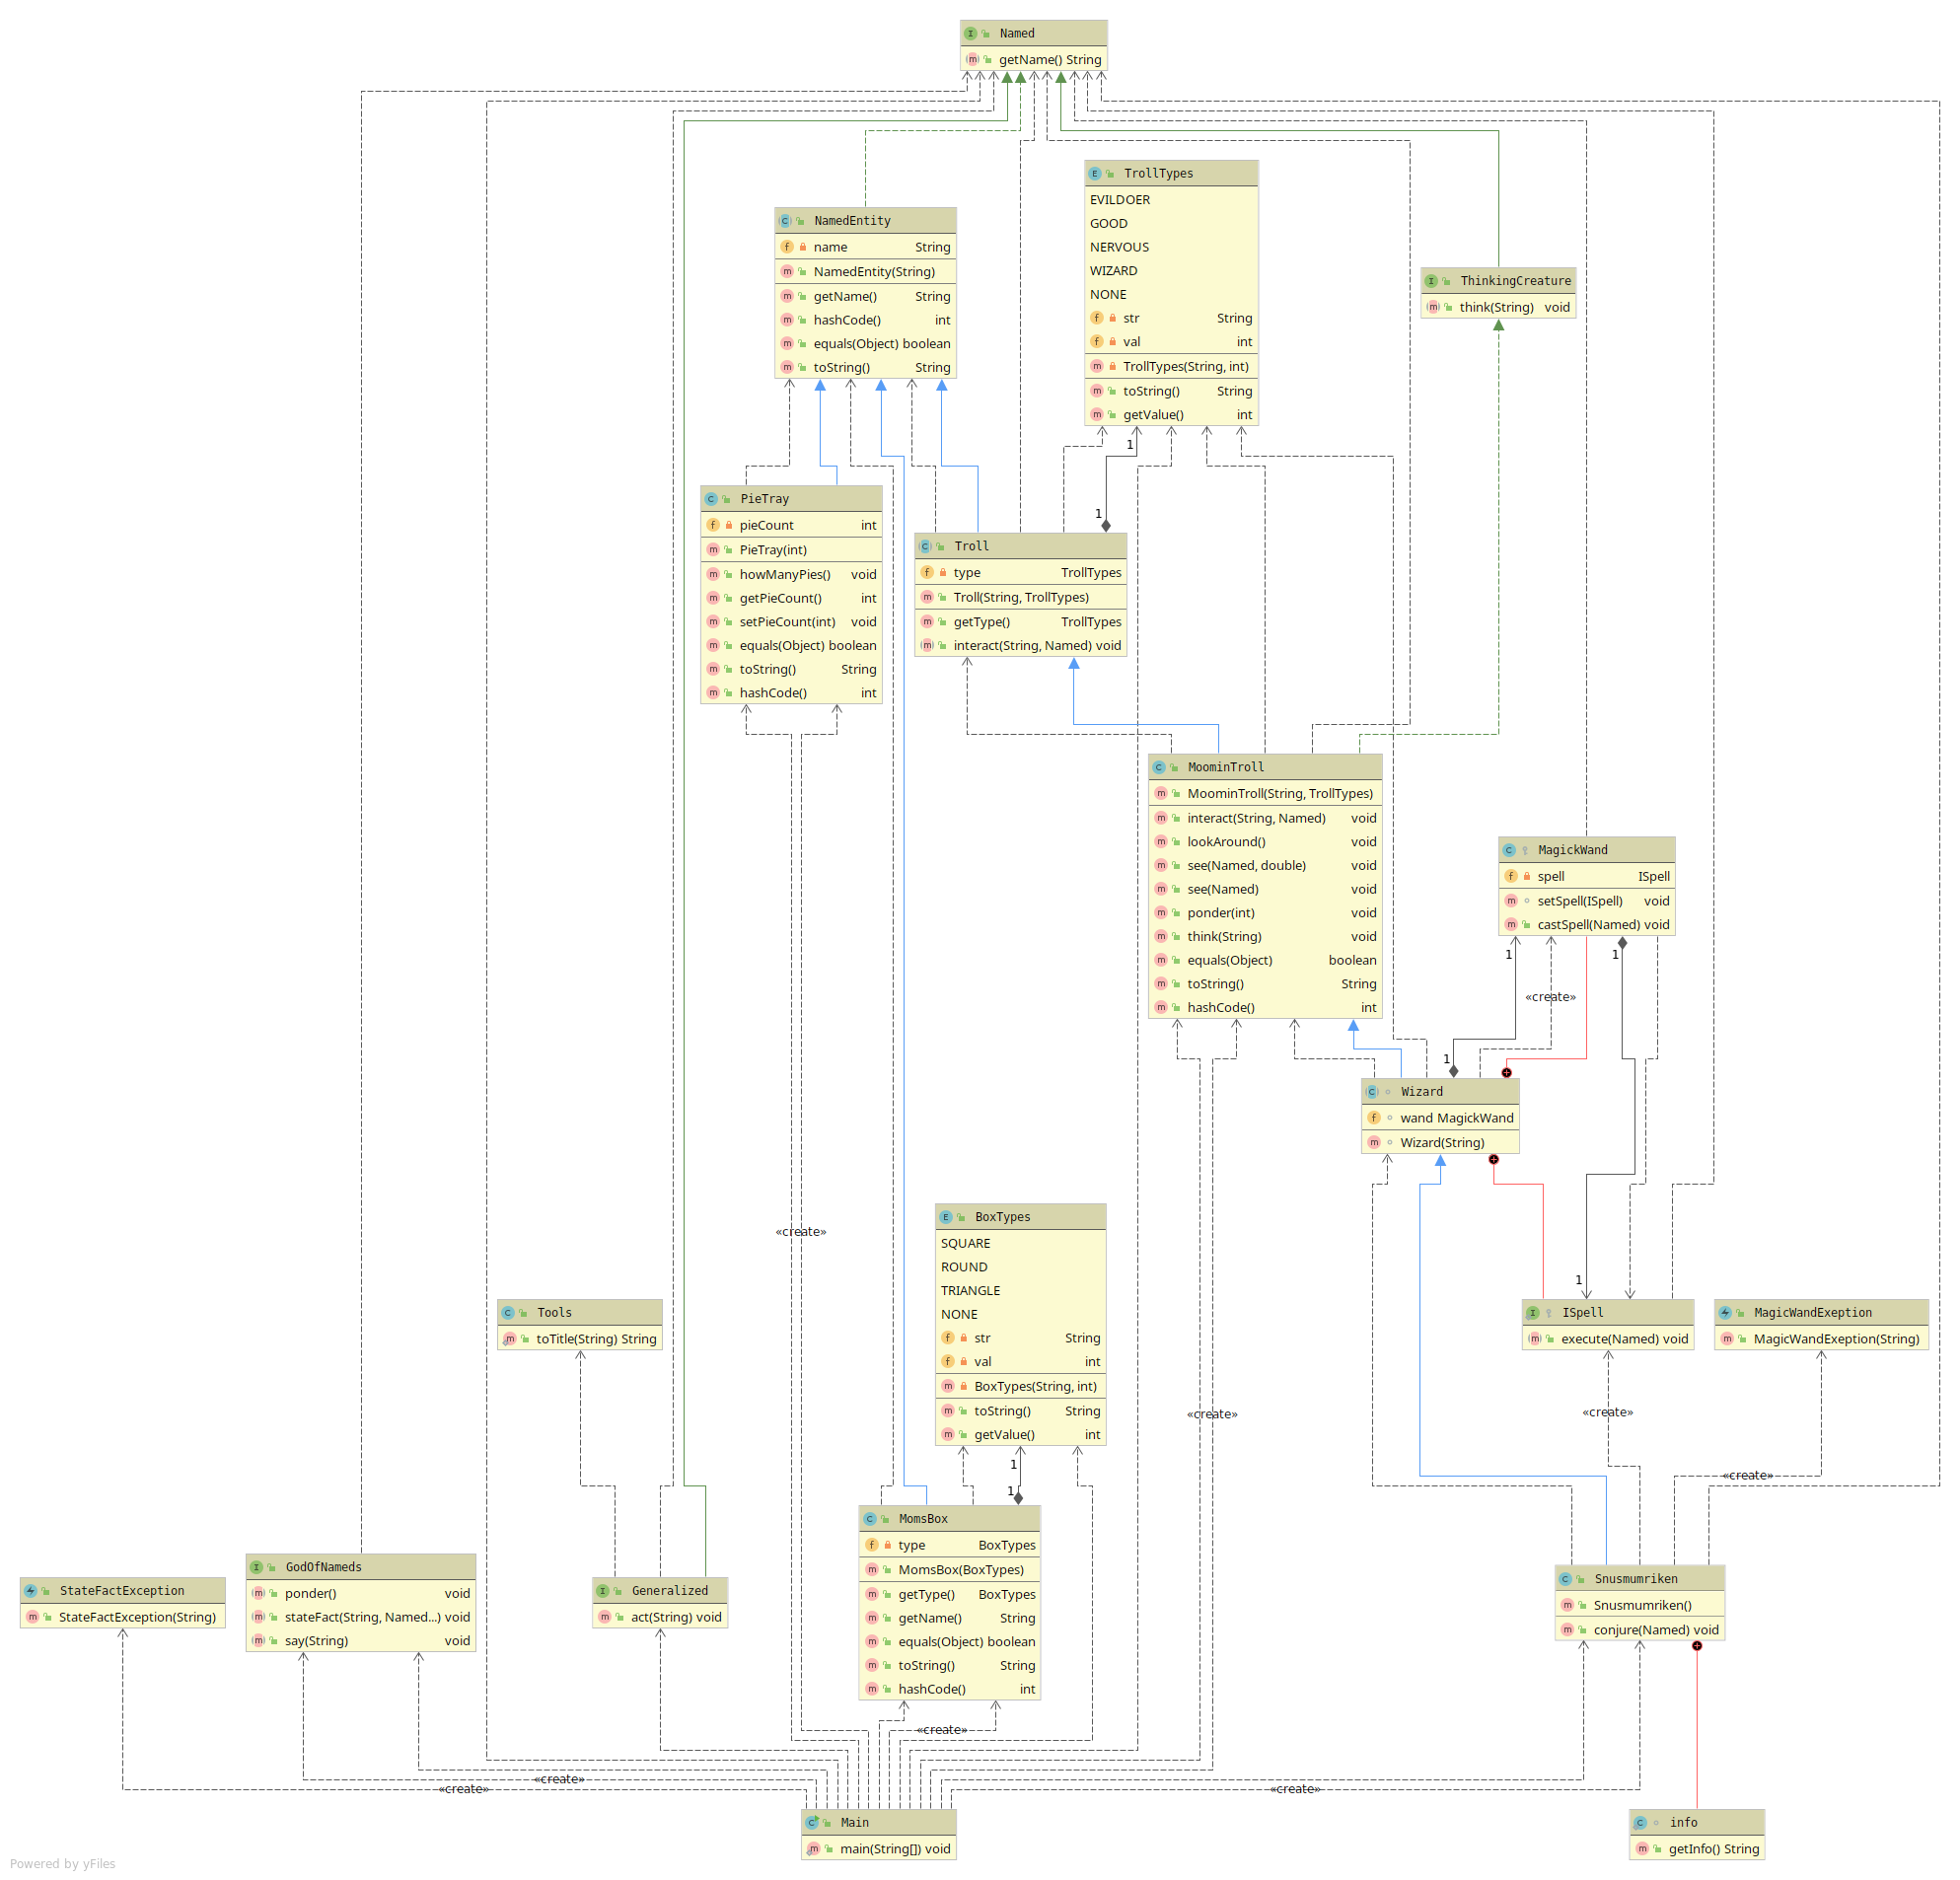
\includegraphics[width=\linewidth]{../dia.png}
  \section{Исходный код программы}
    Исходный код доступен в следующем репозитории:
    
     \href{https://github.com/kupp1/itmo_labs/tree/master/prog/4/prog4lab}{https://github.com/kupp1/itmo\_labs/tree/master/prog/4/prog4lab}
     \begin{figure}[H]
     	\centering
     	 
\includegraphics[scale=0.3155]{../link.png}
     \end{figure}
 \section{Результат работы программы}
	 \footnotesize
 	\inputminted[linenos=true, breaklines=true]{text}{../out.txt}
 \section{Вывод}
 \normalsize
 В ходе этой лабораторной работы я доработал свою объектную модель из предыдущей лабораторной, добавив в неё новые элементы (если честно, то просто реализовал отношения между объектами, которые описываются простынкой в 300 слов и лучше мне от этого не стало), а так же реализовал локальные, анонимные, вложенные классы. Реализовал два своих класса ошибок, проверяемых и не проверяемых и их обработку (что кажется и есть цель лабораторной.... но кому какое дело, простынку же важнее реализовать, да?).
\end{document}